% !TEX root = ../notes_unsupervisedlearning.tex
% Chapter 10: Weak Supervision and Labeling Functions
%%%%%%%%%%%%%%%%%%%%%%%%%%%%%%%%%%%%%%%%%%%%%%%%%%%%%%%%%%%%%%%%%%%%%%

\chapter{Weak Supervision and Labeling Functions}\index{Weak Supervision}\index{Snorkel}
\newthought{What if labels are noisy, partial, or heuristic?}

%═══════════════════════════════════════════════════════════════════════
% BLOCK 1: INTRODUCTION
%═══════════════════════════════════════════════════════════════════════

\section{The Why}

\marginnote{Labels are random variables, not ground truth facts.}

The assumption of clean labels is a fiction:
\begin{itemize}
    \item \textbf{Crowd workers} make mistakes (5--20\% error rates common)
    \item \textbf{Experts disagree} on ambiguous cases
    \item \textbf{Heuristics} provide cheap but noisy labels
    \item \textbf{Legacy data} has inconsistent labeling standards
\end{itemize}

Rather than pretend labels are perfect, \textbf{weak supervision} embraces noise:
\begin{itemize}
    \item Model label uncertainty explicitly
    \item Combine multiple noisy sources
    \item Learn despite imperfect supervision
\end{itemize}

\subsection{Hands-On Experience}

\begin{marginfigure}
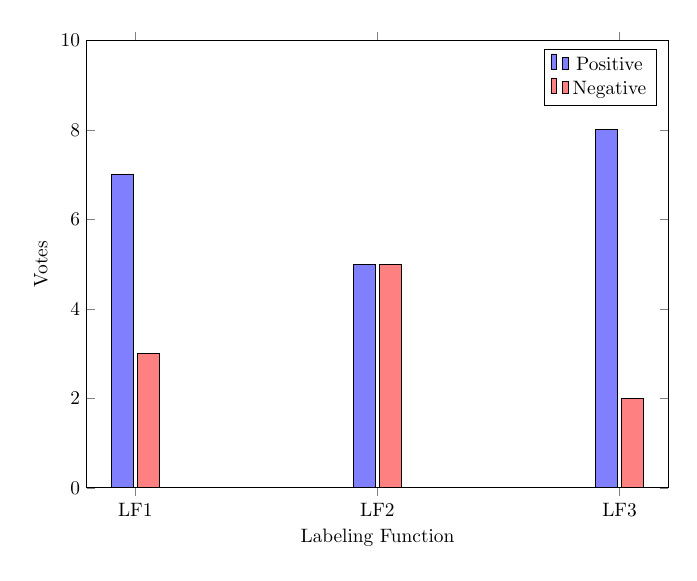
\begin{tikzpicture}[scale=0.7]
    \begin{axis}[
        ybar,
        xlabel={Labeling Function},
        ylabel={Votes},
        ymin=0, ymax=10,
        xtick={1,2,3},
        xticklabels={LF1, LF2, LF3},
        width=\textwidth,
        height=0.8\textwidth,
        bar width=0.4cm,
    ]
    \addplot[fill=blue!50] coordinates {(1,7) (2,5) (3,8)};
    \addplot[fill=red!50] coordinates {(1,3) (2,5) (3,2)};
    \legend{Positive, Negative}
    \end{axis}
\end{tikzpicture}
\caption{Three labeling functions voting on examples. They disagree!}
\end{marginfigure}

You want to classify emails as spam/not-spam. You write three rules:
\begin{enumerate}
    \item LF1: Contains "free money" $\to$ spam
    \item LF2: From known contact $\to$ not spam
    \item LF3: Contains link + urgency words $\to$ spam
\end{enumerate}

For an email from a known contact about a "free trial offer":
\begin{itemize}
    \item LF1 votes: spam (matches "free")
    \item LF2 votes: not spam (known contact)
    \item LF3 votes: abstain (no link)
\end{itemize}

How do you combine these conflicting votes?

\subsection{Learning Objectives}

After this lecture, you will be able to:
\begin{enumerate}
    \item Design labeling functions that encode domain knowledge
    \item Model labeler accuracy and correlation in a label model
    \item Apply the Snorkel framework for programmatic labeling
    \item Handle label noise through loss correction and sample weighting
    \item Combine multiple weak supervision sources
\end{enumerate}

%═══════════════════════════════════════════════════════════════════════
% BLOCK 2: MAIN THEORY
%═══════════════════════════════════════════════════════════════════════

\section{Sources of Weak Labels}

\marginnote{Weak labels come from many sources, each with different characteristics.}

\begin{table}[h]
\centering
\begin{tabular}{lcc}
\toprule
\textbf{Source} & \textbf{Coverage} & \textbf{Accuracy} \\
\midrule
Expert annotation & High & High (95\%+) \\
Crowd workers & High & Medium (70--90\%) \\
Heuristic rules & Low--Medium & Variable \\
Distant supervision & High & Low--Medium \\
Pre-trained models & High & Medium--High \\
\bottomrule
\end{tabular}
\caption{Common weak supervision sources}
\end{table}

\begin{description}
    \item[Noisy crowd labels] Multiple annotators with varying quality
    \item[Distant supervision] Labels from knowledge bases (e.g., all sentences mentioning two entities in a relation $\to$ express that relation)
    \item[Heuristic rules] Domain knowledge encoded as functions
    \item[Data augmentation] Transformed examples inherit parent labels
    \item[Auxiliary signals] Metadata, user behavior, sensor data
\end{description}


\section{Labeling Functions}

\marginnote{A labeling function is a noisy voter that may abstain.}

\begin{definition}[Labeling Function]
A labeling function $\lambda: X \to Y \cup \{\emptyset\}$ maps inputs to a label or abstention ($\emptyset$).
\end{definition}

\textbf{Examples for text classification}:
\begin{itemize}
    \item Keyword matching: contains("urgent") $\to$ spam
    \item Pattern matching: regex for phone numbers $\to$ contact info
    \item External models: sentiment classifier output
    \item Heuristics: short emails $\to$ not spam
\end{itemize}

\subsection{Properties of Good Labeling Functions}

\begin{itemize}
    \item \textbf{High precision}: When it votes, it's usually right
    \item \textbf{Reasonable coverage}: Votes on enough examples
    \item \textbf{Diverse}: Different LFs capture different patterns
    \item \textbf{Low correlation}: Errors are independent
\end{itemize}

\begin{figure}[h]
\centering
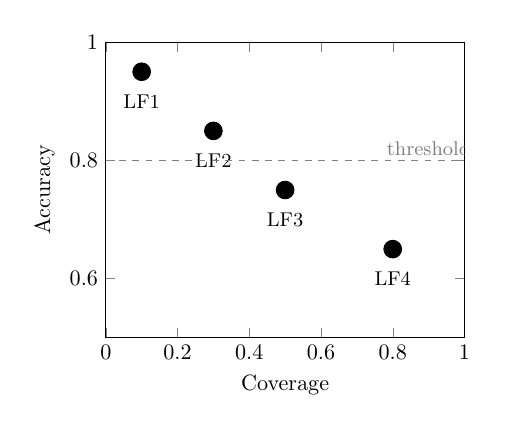
\begin{tikzpicture}[scale=0.8]
    \begin{axis}[
        xlabel={Coverage},
        ylabel={Accuracy},
        xmin=0, xmax=1,
        ymin=0.5, ymax=1,
        width=0.6\textwidth,
    ]
    \addplot[only marks, mark=*, mark size=4pt] coordinates {
        (0.1, 0.95) (0.3, 0.85) (0.5, 0.75) (0.8, 0.65)
    };
    \node at (axis cs:0.1, 0.9) {\small LF1};
    \node at (axis cs:0.3, 0.8) {\small LF2};
    \node at (axis cs:0.5, 0.7) {\small LF3};
    \node at (axis cs:0.8, 0.6) {\small LF4};
    \draw[dashed, gray] (axis cs:0,0.8) -- (axis cs:1,0.8);
    \node[gray] at (axis cs:0.9, 0.82) {\small threshold};
    \end{axis}
\end{tikzpicture}
\caption{Labeling functions trade off coverage and accuracy.}
\end{figure}


\section{Label Modeling}

\marginnote{The label model estimates true labels from noisy votes.}

\subsection{Majority Vote (Baseline)}

Simple aggregation:
\begin{equation}
    \hat{y} = \text{mode}(\{\lambda_i(x) : \lambda_i(x) \neq \emptyset\})
\end{equation}

\textbf{Problems}: Assumes equal accuracy, ignores correlations.

\subsection{Modeling Labeler Accuracy}

Treat each LF as having accuracy $\alpha_i = P(\lambda_i(x) = y | \lambda_i(x) \neq \emptyset)$.

Weighted vote:
\begin{equation}
    P(y | \lambda_1, \ldots, \lambda_m) \propto P(y) \prod_{i: \lambda_i \neq \emptyset} P(\lambda_i | y)
\end{equation}

\subsection{Modeling Correlations}

Labeling functions may have correlated errors (e.g., two keyword-based LFs fail on the same examples).

Factor graph model:
\begin{equation}
    P(y, \lambda_1, \ldots, \lambda_m) = \frac{1}{Z} \phi_Y(y) \prod_i \phi_i(y, \lambda_i) \prod_{i,j} \phi_{ij}(\lambda_i, \lambda_j)
\end{equation}

where $\phi_{ij}$ captures pairwise correlations.


\section{The Snorkel Framework}

\marginnote{Snorkel: end-to-end weak supervision system (Ratner et al., 2017)}

\begin{figure}[h]
\centering
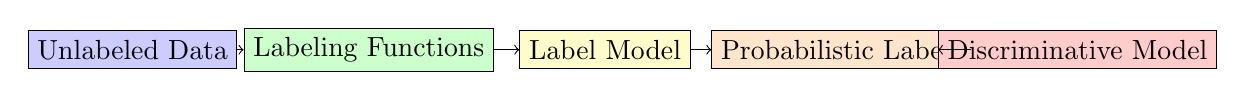
\begin{tikzpicture}[node distance=1.5cm]
    \node[draw, rectangle, fill=blue!20] (data) {Unlabeled Data};
    \node[draw, rectangle, right of=data, xshift=1.5cm, fill=green!20] (lfs) {Labeling Functions};
    \node[draw, rectangle, right of=lfs, xshift=1.5cm, fill=yellow!20] (lm) {Label Model};
    \node[draw, rectangle, right of=lm, xshift=1.5cm, fill=orange!20] (prob) {Probabilistic Labels};
    \node[draw, rectangle, right of=prob, xshift=1.5cm, fill=red!20] (dm) {Discriminative Model};

    \draw[->] (data) -- (lfs);
    \draw[->] (lfs) -- (lm);
    \draw[->] (lm) -- (prob);
    \draw[->] (prob) -- (dm);
\end{tikzpicture}
\caption{Snorkel pipeline: LFs $\to$ Label Model $\to$ Probabilistic Labels $\to$ Train End Model}
\end{figure}

\begin{algorithm}[H]
\caption{Snorkel Workflow}
\begin{algorithmic}[1]
\State \textbf{Write} labeling functions encoding domain knowledge
\State \textbf{Apply} LFs to unlabeled data $\to$ label matrix $\Lambda$
\State \textbf{Train} label model on $\Lambda$ to estimate LF accuracies/correlations
\State \textbf{Generate} probabilistic labels $\tilde{y} = P(y | \Lambda)$
\State \textbf{Train} discriminative model on $(X, \tilde{y})$
\end{algorithmic}
\end{algorithm}

\textbf{Key insight}: The discriminative model generalizes beyond the labeling functions---it learns features, not just rules.


\section{Learning with Label Noise}

\marginnote{Even with probabilistic labels, training can be noisy.}

\subsection{Forward/Backward Loss Correction}

If noise is class-conditional with known transition matrix $T$ where $T_{ij} = P(\tilde{y} = j | y = i)$:

\textbf{Forward correction}:
\begin{equation}
    \tilde{\ell}(f(x), \tilde{y}) = \ell(f(x), T^T f(x))
\end{equation}

\textbf{Backward correction}:
\begin{equation}
    \tilde{\ell}(f(x), \tilde{y}) = T^{-1} \ell(f(x), \tilde{y})
\end{equation}

\subsection{Sample Weighting}

Down-weight likely-mislabeled examples:
\begin{equation}
    \mathcal{L} = \sum_i w_i \ell(f(x_i), \tilde{y}_i)
\end{equation}

where $w_i$ is based on loss value, prediction confidence, or label model confidence.

\subsection{Co-Teaching}

Train two networks; each selects small-loss samples for the other:
\begin{itemize}
    \item Network A selects clean samples for Network B
    \item Network B selects clean samples for Network A
    \item Both avoid memorizing the same noisy labels
\end{itemize}


\section{Association Rules as Labeling Functions}

\marginnote{From Apriori to labeling: mine rules from data structure.}

\textbf{Connection to association rule learning}:
\begin{itemize}
    \item Association rules: $\{A, B\} \to \{C\}$ with support and confidence
    \item Labeling functions: $\text{condition}(x) \to \text{label}$
\end{itemize}

Mining frequent patterns can automatically generate labeling functions:
\begin{enumerate}
    \item Find frequent itemsets in feature space
    \item Convert to rules with confidence threshold
    \item Use as labeling functions
\end{enumerate}


%═══════════════════════════════════════════════════════════════════════
% BLOCK 3: STUDENT ACTIVATION
%═══════════════════════════════════════════════════════════════════════

\section{Examples \& Exercises}

\subsection{Exercise 1: Write Labeling Functions}

Design 5 labeling functions for classifying product reviews as positive/negative:

\textbf{Solution}:
\begin{enumerate}
    \item Contains "love", "amazing", "great" $\to$ positive
    \item Contains "hate", "terrible", "awful" $\to$ negative
    \item Rating $\geq$ 4 stars (if available) $\to$ positive
    \item Review length $<$ 10 words + exclamation $\to$ positive
    \item Contains "return", "refund", "broken" $\to$ negative
\end{enumerate}

\subsection{Exercise 2: Label Aggregation}

Three LFs vote on an example:
\begin{itemize}
    \item LF1: positive (accuracy 0.9)
    \item LF2: negative (accuracy 0.8)
    \item LF3: positive (accuracy 0.7)
\end{itemize}

Assuming independent LFs and uniform prior, compute $P(y = \text{positive})$.

\textbf{Solution}:
\begin{align*}
    P(+|\lambda) &\propto P(+) \cdot P(\lambda_1=+|+) \cdot P(\lambda_2=-|+) \cdot P(\lambda_3=+|+) \\
    &\propto 0.5 \cdot 0.9 \cdot 0.2 \cdot 0.7 = 0.063 \\
    P(-|\lambda) &\propto 0.5 \cdot 0.1 \cdot 0.8 \cdot 0.3 = 0.012 \\
    P(+|\lambda) &= 0.063 / (0.063 + 0.012) = 0.84
\end{align*}

\subsection{Exercise 3: LF Correlation}

Two LFs both use keyword matching. Why might their errors be correlated? How does this affect the label model?

\textbf{Solution}: Both fail on sarcasm, negation, or domain-specific language. If the label model assumes independence, it overestimates combined accuracy. Modeling correlation prevents double-counting evidence.


\section{Self-Reflection \& Recap}

\subsection{Reflection Questions}
\begin{enumerate}
    \item When is weak supervision preferable to collecting clean labels?
    \begin{quote}
        \textit{When labeling is expensive/slow, domain expertise is scarce, or you need to iterate quickly. Also when the task is well-defined by rules.}
    \end{quote}

    \item How do you know if your labeling functions are good enough?
    \begin{quote}
        \textit{Check coverage, estimated accuracy, and conflicts. Validate on a small held-out labeled set. Monitor end model performance.}
    \end{quote}
\end{enumerate}

\subsection{Key Concepts}
\begin{itemize}
    \item \textbf{Weak supervision} scales labeling through programmatic approaches
    \item \textbf{Labeling functions} encode domain knowledge as noisy voters
    \item \textbf{Label models} aggregate noisy sources into probabilistic labels
    \item \textbf{Snorkel} provides an end-to-end framework
    \item \textbf{Noise-robust training} handles remaining label errors
\end{itemize}

\subsection{Next Chapter Teaser}
\marginnote{Teaser: From external labels to self-labels}
\newthought{We've used heuristics and noisy sources for labels.} But what if the model itself becomes the labeler? The next chapter explores \textbf{self-training}: using the model's own predictions as training signal.
